\documentclass[1p]{elsarticle_modified}
%\bibliographystyle{elsarticle-num}

%\usepackage[colorlinks]{hyperref}
%\usepackage{abbrmath_seonhwa} %\Abb, \Ascr, \Acal ,\Abf, \Afrak
\usepackage{amsfonts}
\usepackage{amssymb}
\usepackage{amsmath}
\usepackage{amsthm}
\usepackage{scalefnt}
\usepackage{amsbsy}
\usepackage{kotex}
\usepackage{caption}
\usepackage{subfig}
\usepackage{color}
\usepackage{graphicx}
\usepackage{xcolor} %% white, black, red, green, blue, cyan, magenta, yellow
\usepackage{float}
\usepackage{setspace}
\usepackage{hyperref}

\usepackage{tikz}
\usetikzlibrary{arrows}

\usepackage{multirow}
\usepackage{array} % fixed length table
\usepackage{hhline}

%%%%%%%%%%%%%%%%%%%%%
\makeatletter
\renewcommand*\env@matrix[1][\arraystretch]{%
	\edef\arraystretch{#1}%
	\hskip -\arraycolsep
	\let\@ifnextchar\new@ifnextchar
	\array{*\c@MaxMatrixCols c}}
\makeatother %https://tex.stackexchange.com/questions/14071/how-can-i-increase-the-line-spacing-in-a-matrix
%%%%%%%%%%%%%%%

\usepackage[normalem]{ulem}

\newcommand{\msout}[1]{\ifmmode\text{\sout{\ensuremath{#1}}}\else\sout{#1}\fi}
%SOURCE: \msout is \stkout macro in https://tex.stackexchange.com/questions/20609/strikeout-in-math-mode

\newcommand{\cancel}[1]{
	\ifmmode
	{\color{red}\msout{#1}}
	\else
	{\color{red}\sout{#1}}
	\fi
}

\newcommand{\add}[1]{
	{\color{blue}\uwave{#1}}
}

\newcommand{\replace}[2]{
	\ifmmode
	{\color{red}\msout{#1}}{\color{blue}\uwave{#2}}
	\else
	{\color{red}\sout{#1}}{\color{blue}\uwave{#2}}
	\fi
}

\newcommand{\Sol}{\mathcal{S}} %segment
\newcommand{\D}{D} %diagram
\newcommand{\A}{\mathcal{A}} %arc


%%%%%%%%%%%%%%%%%%%%%%%%%%%%%5 test

\def\sl{\operatorname{\textup{SL}}(2,\Cbb)}
\def\psl{\operatorname{\textup{PSL}}(2,\Cbb)}
\def\quan{\mkern 1mu \triangleright \mkern 1mu}

\theoremstyle{definition}
\newtheorem{thm}{Theorem}[section]
\newtheorem{prop}[thm]{Proposition}
\newtheorem{lem}[thm]{Lemma}
\newtheorem{ques}[thm]{Question}
\newtheorem{cor}[thm]{Corollary}
\newtheorem{defn}[thm]{Definition}
\newtheorem{exam}[thm]{Example}
\newtheorem{rmk}[thm]{Remark}
\newtheorem{alg}[thm]{Algorithm}

\newcommand{\I}{\sqrt{-1}}
\begin{document}

%\begin{frontmatter}
%
%\title{Boundary parabolic representations of knots up to 8 crossings}
%
%%% Group authors per affiliation:
%\author{Yunhi Cho} 
%\address{Department of Mathematics, University of Seoul, Seoul, Korea}
%\ead{yhcho@uos.ac.kr}
%
%
%\author{Seonhwa Kim} %\fnref{s_kim}}
%\address{Center for Geometry and Physics, Institute for Basic Science, Pohang, 37673, Korea}
%\ead{ryeona17@ibs.re.kr}
%
%\author{Hyuk Kim}
%\address{Department of Mathematical Sciences, Seoul National University, Seoul 08826, Korea}
%\ead{hyukkim@snu.ac.kr}
%
%\author{Seokbeom Yoon}
%\address{Department of Mathematical Sciences, Seoul National University, Seoul, 08826,  Korea}
%\ead{sbyoon15@snu.ac.kr}
%
%\begin{abstract}
%We find all boundary parabolic representation of knots up to 8 crossings.
%
%\end{abstract}
%\begin{keyword}
%    \MSC[2010] 57M25 
%\end{keyword}
%
%\end{frontmatter}

%\linenumbers
%\tableofcontents
%
\newcommand\colored[1]{\textcolor{white}{\rule[-0.35ex]{0.8em}{1.4ex}}\kern-0.8em\color{red} #1}%
%\newcommand\colored[1]{\textcolor{white}{ #1}\kern-2.17ex	\textcolor{white}{ #1}\kern-1.81ex	\textcolor{white}{ #1}\kern-2.15ex\color{red}#1	}

{\Large $\underline{12a_{0404}~(K12a_{0404})}$}

\setlength{\tabcolsep}{10pt}
\renewcommand{\arraystretch}{1.6}
\vspace{1cm}\begin{tabular}{m{100pt}>{\centering\arraybackslash}m{274pt}}
\multirow{5}{120pt}{
	\centering
	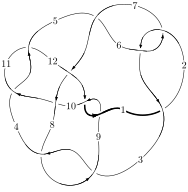
\includegraphics[width=112pt]{../../../GIT/diagram.site/Diagrams/png/1205_12a_0404.png}\\
\ \ \ A knot diagram\footnotemark}&
\allowdisplaybreaks
\textbf{Linearized knot diagam} \\
\cline{2-2}
 &
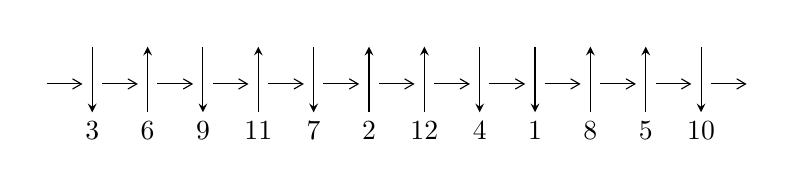
\begin{tikzpicture}[x=20pt, y=17pt]
	% nodes
	\node (C0) at (0, 0) {};
	\node (C1) at (1, 0) {};
	\node (C1U) at (1, +1) {};
	\node (C1D) at (1, -1) {3};

	\node (C2) at (2, 0) {};
	\node (C2U) at (2, +1) {};
	\node (C2D) at (2, -1) {6};

	\node (C3) at (3, 0) {};
	\node (C3U) at (3, +1) {};
	\node (C3D) at (3, -1) {9};

	\node (C4) at (4, 0) {};
	\node (C4U) at (4, +1) {};
	\node (C4D) at (4, -1) {11};

	\node (C5) at (5, 0) {};
	\node (C5U) at (5, +1) {};
	\node (C5D) at (5, -1) {7};

	\node (C6) at (6, 0) {};
	\node (C6U) at (6, +1) {};
	\node (C6D) at (6, -1) {2};

	\node (C7) at (7, 0) {};
	\node (C7U) at (7, +1) {};
	\node (C7D) at (7, -1) {12};

	\node (C8) at (8, 0) {};
	\node (C8U) at (8, +1) {};
	\node (C8D) at (8, -1) {4};

	\node (C9) at (9, 0) {};
	\node (C9U) at (9, +1) {};
	\node (C9D) at (9, -1) {1};

	\node (C10) at (10, 0) {};
	\node (C10U) at (10, +1) {};
	\node (C10D) at (10, -1) {8};

	\node (C11) at (11, 0) {};
	\node (C11U) at (11, +1) {};
	\node (C11D) at (11, -1) {5};

	\node (C12) at (12, 0) {};
	\node (C12U) at (12, +1) {};
	\node (C12D) at (12, -1) {10};
	\node (C13) at (13, 0) {};

	% arrows
	\draw[->,>={angle 60}]
	(C0) edge (C1) (C1) edge (C2) (C2) edge (C3) (C3) edge (C4) (C4) edge (C5) (C5) edge (C6) (C6) edge (C7) (C7) edge (C8) (C8) edge (C9) (C9) edge (C10) (C10) edge (C11) (C11) edge (C12) (C12) edge (C13) ;	\draw[->,>=stealth]
	(C1U) edge (C1D) (C2D) edge (C2U) (C3U) edge (C3D) (C4D) edge (C4U) (C5U) edge (C5D) (C6D) edge (C6U) (C7D) edge (C7U) (C8U) edge (C8D) (C9U) edge (C9D) (C10D) edge (C10U) (C11D) edge (C11U) (C12U) edge (C12D) ;
	\end{tikzpicture} \\
\hhline{~~} \\& 
\textbf{Solving Sequence} \\ \cline{2-2} 
 &
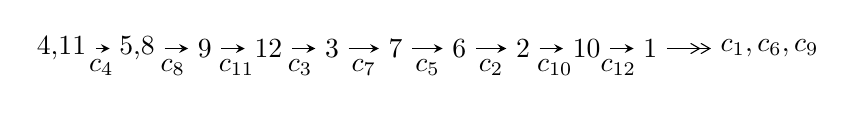
\begin{tikzpicture}[x=23pt, y=7pt]
	% node
	\node (A0) at (-1/8, 0) {4,11};
	\node (A1) at (17/16, 0) {5,8};
	\node (A2) at (17/8, 0) {9};
	\node (A3) at (25/8, 0) {12};
	\node (A4) at (33/8, 0) {3};
	\node (A5) at (41/8, 0) {7};
	\node (A6) at (49/8, 0) {6};
	\node (A7) at (57/8, 0) {2};
	\node (A8) at (65/8, 0) {10};
	\node (A9) at (73/8, 0) {1};
	\node (C1) at (1/2, -1) {$c_{4}$};
	\node (C2) at (13/8, -1) {$c_{8}$};
	\node (C3) at (21/8, -1) {$c_{11}$};
	\node (C4) at (29/8, -1) {$c_{3}$};
	\node (C5) at (37/8, -1) {$c_{7}$};
	\node (C6) at (45/8, -1) {$c_{5}$};
	\node (C7) at (53/8, -1) {$c_{2}$};
	\node (C8) at (61/8, -1) {$c_{10}$};
	\node (C9) at (69/8, -1) {$c_{12}$};
	\node (A10) at (11, 0) {$c_{1},c_{6},c_{9}$};

	% edge
	\draw[->,>=stealth]	
	(A0) edge (A1) (A1) edge (A2) (A2) edge (A3) (A3) edge (A4) (A4) edge (A5) (A5) edge (A6) (A6) edge (A7) (A7) edge (A8) (A8) edge (A9) ;
	\draw[->>,>={angle 60}]	
	(A9) edge (A10);
\end{tikzpicture} \\ 

\end{tabular} \\

\footnotetext{
The image of knot diagram is generated by the software ``\textbf{Draw programme}" developed by Andrew Bartholomew(\url{http://www.layer8.co.uk/maths/draw/index.htm\#Running-draw}), where we modified some parts for our purpose(\url{https://github.com/CATsTAILs/LinksPainter}).
}\phantom \\ \newline 
\centering \textbf{Ideals for irreducible components\footnotemark of $X_{\text{par}}$} 
 
\begin{align*}
I^u_{1}&=\langle 
2.48423\times10^{353} u^{108}-1.06966\times10^{353} u^{107}+\cdots+3.86962\times10^{353} b+5.71739\times10^{352},\\
\phantom{I^u_{1}}&\phantom{= \langle  }-1.59044\times10^{353} u^{108}+2.79797\times10^{352} u^{107}+\cdots+3.86962\times10^{353} a+3.48502\times10^{353},\\
\phantom{I^u_{1}}&\phantom{= \langle  }u^{109}+u^{108}+\cdots+2 u-1\rangle \\
I^u_{2}&=\langle 
-37327 u^{29}+401711 u^{28}+\cdots+361945 b-312854,\\
\phantom{I^u_{2}}&\phantom{= \langle  }-496929 u^{29}+205552 u^{28}+\cdots+361945 a-554238,\;u^{30}-11 u^{28}+\cdots-11 u^2+1\rangle \\
\\
\end{align*}
\raggedright * 2 irreducible components of $\dim_{\mathbb{C}}=0$, with total 139 representations.\\
\footnotetext{All coefficients of polynomials are rational numbers. But the coefficients are sometimes approximated in decimal forms when there is not enough margin.}
\newpage
\renewcommand{\arraystretch}{1}
\centering \section*{I. $I^u_{1}= \langle 2.48\times10^{353} u^{108}-1.07\times10^{353} u^{107}+\cdots+3.87\times10^{353} b+5.72\times10^{352},\;-1.59\times10^{353} u^{108}+2.80\times10^{352} u^{107}+\cdots+3.87\times10^{353} a+3.49\times10^{353},\;u^{109}+u^{108}+\cdots+2 u-1 \rangle$}
\flushleft \textbf{(i) Arc colorings}\\
\begin{tabular}{m{7pt} m{180pt} m{7pt} m{180pt} }
\flushright $a_{4}=$&$\begin{pmatrix}1\\0\end{pmatrix}$ \\
\flushright $a_{11}=$&$\begin{pmatrix}0\\u\end{pmatrix}$ \\
\flushright $a_{5}=$&$\begin{pmatrix}1\\- u^2\end{pmatrix}$ \\
\flushright $a_{8}=$&$\begin{pmatrix}0.411008 u^{108}-0.0723061 u^{107}+\cdots+70.2222 u-0.900610\\-0.641982 u^{108}+0.276426 u^{107}+\cdots-17.2430 u-0.147751\end{pmatrix}$ \\
\flushright $a_{9}=$&$\begin{pmatrix}1.05299 u^{108}-0.348732 u^{107}+\cdots+87.4652 u-0.752859\\-0.641982 u^{108}+0.276426 u^{107}+\cdots-17.2430 u-0.147751\end{pmatrix}$ \\
\flushright $a_{12}=$&$\begin{pmatrix}u\\- u^3+u\end{pmatrix}$ \\
\flushright $a_{3}=$&$\begin{pmatrix}-0.146173 u^{108}+0.0919442 u^{107}+\cdots-91.2533 u-10.0700\\0.193937 u^{108}-0.261341 u^{107}+\cdots+2.37985 u+0.482388\end{pmatrix}$ \\
\flushright $a_{7}=$&$\begin{pmatrix}1.12746 u^{108}-0.401791 u^{107}+\cdots+72.3535 u-1.66265\\-1.13976 u^{108}+0.503579 u^{107}+\cdots-17.9201 u+0.136140\end{pmatrix}$ \\
\flushright $a_{6}=$&$\begin{pmatrix}-0.0937440 u^{108}+0.313213 u^{107}+\cdots+80.1708 u+14.1735\\0.553987 u^{108}-0.438620 u^{107}+\cdots+0.869280 u-1.66470\end{pmatrix}$ \\
\flushright $a_{2}=$&$\begin{pmatrix}0.929411 u^{108}-0.488793 u^{107}+\cdots-120.689 u-2.98918\\-1.13520 u^{108}+0.440053 u^{107}+\cdots+19.8376 u+2.19256\end{pmatrix}$ \\
\flushright $a_{10}=$&$\begin{pmatrix}-0.710297 u^{108}-1.39387 u^{107}+\cdots+67.3057 u+1.35505\\-0.217162 u^{108}+0.149794 u^{107}+\cdots-9.68315 u+0.0477646\end{pmatrix}$ \\
\flushright $a_{1}=$&$\begin{pmatrix}-0.590162 u^{108}-0.0598138 u^{107}+\cdots+71.6155 u+3.50080\\0.363252 u^{108}-0.00278651 u^{107}+\cdots-16.4705 u-0.204961\end{pmatrix}$\\&\end{tabular}
\flushleft \textbf{(ii) Obstruction class $= -1$}\\~\\
\flushleft \textbf{(iii) Cusp Shapes $= -0.363790 u^{108}+0.673083 u^{107}+\cdots+18.1091 u+10.0328$}\\~\\
\newpage\renewcommand{\arraystretch}{1}
\flushleft \textbf{(iv) u-Polynomials at the component}\newline \\
\begin{tabular}{m{50pt}|m{274pt}}
Crossings & \hspace{64pt}u-Polynomials at each crossing \\
\hline $$\begin{aligned}c_{1},c_{5}\end{aligned}$$&$\begin{aligned}
&u^{109}+31 u^{108}+\cdots-58 u-1
\end{aligned}$\\
\hline $$\begin{aligned}c_{2},c_{6}\end{aligned}$$&$\begin{aligned}
&u^{109}-3 u^{108}+\cdots-29 u^2-1
\end{aligned}$\\
\hline $$\begin{aligned}c_{3},c_{8}\end{aligned}$$&$\begin{aligned}
&u^{109}+u^{108}+\cdots+36101 u-3718
\end{aligned}$\\
\hline $$\begin{aligned}c_{4},c_{11}\end{aligned}$$&$\begin{aligned}
&u^{109}+u^{108}+\cdots+2 u-1
\end{aligned}$\\
\hline $$\begin{aligned}c_{7}\end{aligned}$$&$\begin{aligned}
&u^{109}-3 u^{108}+\cdots-1747923 u-732778
\end{aligned}$\\
\hline $$\begin{aligned}c_{9},c_{12}\end{aligned}$$&$\begin{aligned}
&u^{109}-5 u^{108}+\cdots+48168 u-4657
\end{aligned}$\\
\hline $$\begin{aligned}c_{10}\end{aligned}$$&$\begin{aligned}
&u^{109}+13 u^{108}+\cdots+7934796 u+816091
\end{aligned}$\\
\hline
\end{tabular}\\~\\
\newpage\renewcommand{\arraystretch}{1}
\flushleft \textbf{(v) Riley Polynomials at the component}\newline \\
\begin{tabular}{m{50pt}|m{274pt}}
Crossings & \hspace{64pt}Riley Polynomials at each crossing \\
\hline $$\begin{aligned}c_{1},c_{5}\end{aligned}$$&$\begin{aligned}
&y^{109}+107 y^{108}+\cdots+486 y-1
\end{aligned}$\\
\hline $$\begin{aligned}c_{2},c_{6}\end{aligned}$$&$\begin{aligned}
&y^{109}+31 y^{108}+\cdots-58 y-1
\end{aligned}$\\
\hline $$\begin{aligned}c_{3},c_{8}\end{aligned}$$&$\begin{aligned}
&y^{109}+109 y^{108}+\cdots-49943387 y-13823524
\end{aligned}$\\
\hline $$\begin{aligned}c_{4},c_{11}\end{aligned}$$&$\begin{aligned}
&y^{109}-87 y^{108}+\cdots-130 y-1
\end{aligned}$\\
\hline $$\begin{aligned}c_{7}\end{aligned}$$&$\begin{aligned}
&y^{109}-55 y^{108}+\cdots+33067800692205 y-536963597284
\end{aligned}$\\
\hline $$\begin{aligned}c_{9},c_{12}\end{aligned}$$&$\begin{aligned}
&y^{109}+91 y^{108}+\cdots-420320624 y-21687649
\end{aligned}$\\
\hline $$\begin{aligned}c_{10}\end{aligned}$$&$\begin{aligned}
&y^{109}-55 y^{108}+\cdots+28553913646086 y-666004520281
\end{aligned}$\\
\hline
\end{tabular}\\~\\
\newpage\flushleft \textbf{(vi) Complex Volumes and Cusp Shapes}
$$\begin{array}{c|c|c}  
\text{Solutions to }I^u_{1}& \I (\text{vol} + \sqrt{-1}CS) & \text{Cusp shape}\\
 \hline 
\begin{aligned}
u &= \phantom{-}0.033343 + 0.996771 I \\
a &= \phantom{-}0.537737 - 1.072490 I \\
b &= \phantom{-}0.204491 - 1.283920 I\end{aligned}
 & \phantom{-}3.09309 + 6.33794 I & \phantom{-0.000000 } 0 \\ \hline\begin{aligned}
u &= \phantom{-}0.033343 - 0.996771 I \\
a &= \phantom{-}0.537737 + 1.072490 I \\
b &= \phantom{-}0.204491 + 1.283920 I\end{aligned}
 & \phantom{-}3.09309 - 6.33794 I & \phantom{-0.000000 } 0 \\ \hline\begin{aligned}
u &= -0.083018 + 0.979645 I \\
a &= \phantom{-}0.065424 - 0.380814 I \\
b &= \phantom{-}0.0798719 + 0.0877287 I\end{aligned}
 & \phantom{-}0.93792 + 2.65570 I & \phantom{-0.000000 } 0 \\ \hline\begin{aligned}
u &= -0.083018 - 0.979645 I \\
a &= \phantom{-}0.065424 + 0.380814 I \\
b &= \phantom{-}0.0798719 - 0.0877287 I\end{aligned}
 & \phantom{-}0.93792 - 2.65570 I & \phantom{-0.000000 } 0 \\ \hline\begin{aligned}
u &= -1.025090 + 0.268911 I \\
a &= -0.689799 - 0.014786 I \\
b &= -0.757790 - 0.052253 I\end{aligned}
 & -0.81682 - 2.68878 I & \phantom{-0.000000 } 0 \\ \hline\begin{aligned}
u &= -1.025090 - 0.268911 I \\
a &= -0.689799 + 0.014786 I \\
b &= -0.757790 + 0.052253 I\end{aligned}
 & -0.81682 + 2.68878 I & \phantom{-0.000000 } 0 \\ \hline\begin{aligned}
u &= -1.078590 + 0.164066 I \\
a &= -0.822935 + 0.208584 I \\
b &= -0.34332 - 1.80976 I\end{aligned}
 & \phantom{-}8.02899 - 0.83663 I & \phantom{-0.000000 } 0 \\ \hline\begin{aligned}
u &= -1.078590 - 0.164066 I \\
a &= -0.822935 - 0.208584 I \\
b &= -0.34332 + 1.80976 I\end{aligned}
 & \phantom{-}8.02899 + 0.83663 I & \phantom{-0.000000 } 0 \\ \hline\begin{aligned}
u &= \phantom{-}1.110560 + 0.019710 I \\
a &= -1.223520 + 0.577324 I \\
b &= -0.412338 + 0.247413 I\end{aligned}
 & \phantom{-}1.93011 - 0.33723 I & \phantom{-0.000000 } 0 \\ \hline\begin{aligned}
u &= \phantom{-}1.110560 - 0.019710 I \\
a &= -1.223520 - 0.577324 I \\
b &= -0.412338 - 0.247413 I\end{aligned}
 & \phantom{-}1.93011 + 0.33723 I & \phantom{-0.000000 } 0\\
 \hline 
 \end{array}$$\newpage$$\begin{array}{c|c|c}  
\text{Solutions to }I^u_{1}& \I (\text{vol} + \sqrt{-1}CS) & \text{Cusp shape}\\
 \hline 
\begin{aligned}
u &= \phantom{-}0.505090 + 0.716391 I \\
a &= \phantom{-}0.124304 + 0.701939 I \\
b &= \phantom{-}0.368446 + 0.667258 I\end{aligned}
 & \phantom{-}0.21516 + 1.88326 I & \phantom{-0.000000 } 0 \\ \hline\begin{aligned}
u &= \phantom{-}0.505090 - 0.716391 I \\
a &= \phantom{-}0.124304 - 0.701939 I \\
b &= \phantom{-}0.368446 - 0.667258 I\end{aligned}
 & \phantom{-}0.21516 - 1.88326 I & \phantom{-0.000000 } 0 \\ \hline\begin{aligned}
u &= \phantom{-}1.15469\phantom{ +0.000000I} \\
a &= \phantom{-}0.655493\phantom{ +0.000000I} \\
b &= \phantom{-}0.654397\phantom{ +0.000000I}\end{aligned}
 & \phantom{-}2.20801\phantom{ +0.000000I} & \phantom{-0.000000 } 0 \\ \hline\begin{aligned}
u &= \phantom{-}0.037929 + 0.843453 I \\
a &= \phantom{-}0.952314 + 0.964303 I \\
b &= \phantom{-}1.090140 + 0.131358 I\end{aligned}
 & \phantom{-}5.68628 - 5.95291 I & \phantom{-0.000000 } 0 \\ \hline\begin{aligned}
u &= \phantom{-}0.037929 - 0.843453 I \\
a &= \phantom{-}0.952314 - 0.964303 I \\
b &= \phantom{-}1.090140 - 0.131358 I\end{aligned}
 & \phantom{-}5.68628 + 5.95291 I & \phantom{-0.000000 } 0 \\ \hline\begin{aligned}
u &= \phantom{-}0.042878 + 0.842993 I \\
a &= -1.010680 + 0.886733 I \\
b &= -1.076100 + 0.241905 I\end{aligned}
 & \phantom{-}5.77083 - 0.16968 I & \phantom{-0.000000 } 0 \\ \hline\begin{aligned}
u &= \phantom{-}0.042878 - 0.842993 I \\
a &= -1.010680 - 0.886733 I \\
b &= -1.076100 - 0.241905 I\end{aligned}
 & \phantom{-}5.77083 + 0.16968 I & \phantom{-0.000000 } 0 \\ \hline\begin{aligned}
u &= -0.758819 + 0.364574 I \\
a &= \phantom{-}0.611325 - 1.207200 I \\
b &= \phantom{-}0.314195 + 0.698740 I\end{aligned}
 & \phantom{-}0.30581 - 4.84419 I & \phantom{-0.000000 } 0 \\ \hline\begin{aligned}
u &= -0.758819 - 0.364574 I \\
a &= \phantom{-}0.611325 + 1.207200 I \\
b &= \phantom{-}0.314195 - 0.698740 I\end{aligned}
 & \phantom{-}0.30581 + 4.84419 I & \phantom{-0.000000 } 0 \\ \hline\begin{aligned}
u &= \phantom{-}1.148220 + 0.202593 I \\
a &= -1.30837 - 0.58788 I \\
b &= -0.394987 + 1.105200 I\end{aligned}
 & \phantom{-}2.16765 + 1.28585 I & \phantom{-0.000000 } 0\\
 \hline 
 \end{array}$$\newpage$$\begin{array}{c|c|c}  
\text{Solutions to }I^u_{1}& \I (\text{vol} + \sqrt{-1}CS) & \text{Cusp shape}\\
 \hline 
\begin{aligned}
u &= \phantom{-}1.148220 - 0.202593 I \\
a &= -1.30837 + 0.58788 I \\
b &= -0.394987 - 1.105200 I\end{aligned}
 & \phantom{-}2.16765 - 1.28585 I & \phantom{-0.000000 } 0 \\ \hline\begin{aligned}
u &= -0.428650 + 0.692382 I \\
a &= \phantom{-}0.536353 - 0.512889 I \\
b &= \phantom{-}0.347468 + 0.369372 I\end{aligned}
 & -2.69258 - 1.01062 I & \phantom{-0.000000 } 0 \\ \hline\begin{aligned}
u &= -0.428650 - 0.692382 I \\
a &= \phantom{-}0.536353 + 0.512889 I \\
b &= \phantom{-}0.347468 - 0.369372 I\end{aligned}
 & -2.69258 + 1.01062 I & \phantom{-0.000000 } 0 \\ \hline\begin{aligned}
u &= \phantom{-}1.175660 + 0.243208 I \\
a &= -0.950702 - 0.275405 I \\
b &= -1.138810 + 0.131806 I\end{aligned}
 & \phantom{-}2.39738 + 6.26878 I & \phantom{-0.000000 } 0 \\ \hline\begin{aligned}
u &= \phantom{-}1.175660 - 0.243208 I \\
a &= -0.950702 + 0.275405 I \\
b &= -1.138810 - 0.131806 I\end{aligned}
 & \phantom{-}2.39738 - 6.26878 I & \phantom{-0.000000 } 0 \\ \hline\begin{aligned}
u &= -0.195336 + 0.739888 I \\
a &= -1.02500 - 1.16001 I \\
b &= -0.05710 - 1.41322 I\end{aligned}
 & \phantom{-}6.17025 - 2.54367 I & \phantom{-}6.56336 + 0. I\phantom{ +0.000000I} \\ \hline\begin{aligned}
u &= -0.195336 - 0.739888 I \\
a &= -1.02500 + 1.16001 I \\
b &= -0.05710 + 1.41322 I\end{aligned}
 & \phantom{-}6.17025 + 2.54367 I & \phantom{-}6.56336 + 0. I\phantom{ +0.000000I} \\ \hline\begin{aligned}
u &= -1.225900 + 0.193652 I \\
a &= -2.08131 + 0.91182 I \\
b &= -0.101223 - 1.307610 I\end{aligned}
 & \phantom{-}5.52271 - 1.93932 I & \phantom{-0.000000 } 0 \\ \hline\begin{aligned}
u &= -1.225900 - 0.193652 I \\
a &= -2.08131 - 0.91182 I \\
b &= -0.101223 + 1.307610 I\end{aligned}
 & \phantom{-}5.52271 + 1.93932 I & \phantom{-0.000000 } 0 \\ \hline\begin{aligned}
u &= \phantom{-}0.197394 + 1.232220 I \\
a &= -0.005870 + 0.582501 I \\
b &= \phantom{-}0.164637 + 1.044850 I\end{aligned}
 & -0.911835 - 1.039600 I & \phantom{-0.000000 } 0\\
 \hline 
 \end{array}$$\newpage$$\begin{array}{c|c|c}  
\text{Solutions to }I^u_{1}& \I (\text{vol} + \sqrt{-1}CS) & \text{Cusp shape}\\
 \hline 
\begin{aligned}
u &= \phantom{-}0.197394 - 1.232220 I \\
a &= -0.005870 - 0.582501 I \\
b &= \phantom{-}0.164637 - 1.044850 I\end{aligned}
 & -0.911835 + 1.039600 I & \phantom{-0.000000 } 0 \\ \hline\begin{aligned}
u &= -1.259570 + 0.031187 I \\
a &= -0.602918 - 0.251555 I \\
b &= -0.82128 + 1.99230 I\end{aligned}
 & \phantom{-}13.75470 - 0.11442 I & \phantom{-0.000000 } 0 \\ \hline\begin{aligned}
u &= -1.259570 - 0.031187 I \\
a &= -0.602918 + 0.251555 I \\
b &= -0.82128 - 1.99230 I\end{aligned}
 & \phantom{-}13.75470 + 0.11442 I & \phantom{-0.000000 } 0 \\ \hline\begin{aligned}
u &= -0.283691 + 1.243630 I \\
a &= -0.566798 - 0.739563 I \\
b &= -0.37226 - 1.48415 I\end{aligned}
 & \phantom{-}11.42350 - 4.92170 I & \phantom{-0.000000 } 0 \\ \hline\begin{aligned}
u &= -0.283691 - 1.243630 I \\
a &= -0.566798 + 0.739563 I \\
b &= -0.37226 + 1.48415 I\end{aligned}
 & \phantom{-}11.42350 + 4.92170 I & \phantom{-0.000000 } 0 \\ \hline\begin{aligned}
u &= -1.154790 + 0.559328 I \\
a &= -0.805570 - 0.091463 I \\
b &= -0.12706 - 1.56388 I\end{aligned}
 & \phantom{-}8.55093 - 2.12626 I & \phantom{-0.000000 } 0 \\ \hline\begin{aligned}
u &= -1.154790 - 0.559328 I \\
a &= -0.805570 + 0.091463 I \\
b &= -0.12706 + 1.56388 I\end{aligned}
 & \phantom{-}8.55093 + 2.12626 I & \phantom{-0.000000 } 0 \\ \hline\begin{aligned}
u &= \phantom{-}1.287480 + 0.042107 I \\
a &= -0.703728 + 0.877715 I \\
b &= -0.25001 - 1.46892 I\end{aligned}
 & \phantom{-}9.38679 + 3.46532 I & \phantom{-0.000000 } 0 \\ \hline\begin{aligned}
u &= \phantom{-}1.287480 - 0.042107 I \\
a &= -0.703728 - 0.877715 I \\
b &= -0.25001 + 1.46892 I\end{aligned}
 & \phantom{-}9.38679 - 3.46532 I & \phantom{-0.000000 } 0 \\ \hline\begin{aligned}
u &= \phantom{-}1.295770 + 0.020833 I \\
a &= \phantom{-}0.589598 - 0.226366 I \\
b &= \phantom{-}0.90012 + 1.92095 I\end{aligned}
 & \phantom{-}13.5553 - 6.0485 I & \phantom{-0.000000 } 0\\
 \hline 
 \end{array}$$\newpage$$\begin{array}{c|c|c}  
\text{Solutions to }I^u_{1}& \I (\text{vol} + \sqrt{-1}CS) & \text{Cusp shape}\\
 \hline 
\begin{aligned}
u &= \phantom{-}1.295770 - 0.020833 I \\
a &= \phantom{-}0.589598 + 0.226366 I \\
b &= \phantom{-}0.90012 - 1.92095 I\end{aligned}
 & \phantom{-}13.5553 + 6.0485 I & \phantom{-0.000000 } 0 \\ \hline\begin{aligned}
u &= \phantom{-}0.221763 + 1.286900 I \\
a &= \phantom{-}0.516905 - 0.750170 I \\
b &= \phantom{-}0.41853 - 1.44734 I\end{aligned}
 & \phantom{-}10.8150 + 11.2570 I & \phantom{-0.000000 } 0 \\ \hline\begin{aligned}
u &= \phantom{-}0.221763 - 1.286900 I \\
a &= \phantom{-}0.516905 + 0.750170 I \\
b &= \phantom{-}0.41853 + 1.44734 I\end{aligned}
 & \phantom{-}10.8150 - 11.2570 I & \phantom{-0.000000 } 0 \\ \hline\begin{aligned}
u &= -1.305220 + 0.050689 I \\
a &= -0.90955 - 1.63853 I \\
b &= \phantom{-}0.192471 + 1.340410 I\end{aligned}
 & \phantom{-}13.7099 - 7.1192 I & \phantom{-0.000000 } 0 \\ \hline\begin{aligned}
u &= -1.305220 - 0.050689 I \\
a &= -0.90955 + 1.63853 I \\
b &= \phantom{-}0.192471 - 1.340410 I\end{aligned}
 & \phantom{-}13.7099 + 7.1192 I & \phantom{-0.000000 } 0 \\ \hline\begin{aligned}
u &= -1.301570 + 0.120960 I \\
a &= \phantom{-}0.918003 - 0.450088 I \\
b &= \phantom{-}0.567160 + 0.449045 I\end{aligned}
 & \phantom{-}4.98023 - 3.29980 I & \phantom{-0.000000 } 0 \\ \hline\begin{aligned}
u &= -1.301570 - 0.120960 I \\
a &= \phantom{-}0.918003 + 0.450088 I \\
b &= \phantom{-}0.567160 - 0.449045 I\end{aligned}
 & \phantom{-}4.98023 + 3.29980 I & \phantom{-0.000000 } 0 \\ \hline\begin{aligned}
u &= \phantom{-}0.687185 + 0.047766 I \\
a &= -0.69676 - 1.61994 I \\
b &= -0.009606 + 0.721615 I\end{aligned}
 & \phantom{-}0.429338 + 0.375073 I & \phantom{-}7.10528 - 0.69344 I \\ \hline\begin{aligned}
u &= \phantom{-}0.687185 - 0.047766 I \\
a &= -0.69676 + 1.61994 I \\
b &= -0.009606 - 0.721615 I\end{aligned}
 & \phantom{-}0.429338 - 0.375073 I & \phantom{-}7.10528 + 0.69344 I \\ \hline\begin{aligned}
u &= -1.318050 + 0.000872 I \\
a &= \phantom{-}0.734081 - 0.802225 I \\
b &= \phantom{-}0.35263 + 1.46855 I\end{aligned}
 & \phantom{-}9.84520 - 2.81978 I & \phantom{-0.000000 } 0\\
 \hline 
 \end{array}$$\newpage$$\begin{array}{c|c|c}  
\text{Solutions to }I^u_{1}& \I (\text{vol} + \sqrt{-1}CS) & \text{Cusp shape}\\
 \hline 
\begin{aligned}
u &= -1.318050 - 0.000872 I \\
a &= \phantom{-}0.734081 + 0.802225 I \\
b &= \phantom{-}0.35263 - 1.46855 I\end{aligned}
 & \phantom{-}9.84520 + 2.81978 I & \phantom{-0.000000 } 0 \\ \hline\begin{aligned}
u &= \phantom{-}1.272920 + 0.365794 I \\
a &= -0.791956 - 0.247182 I \\
b &= -1.60507 + 0.49517 I\end{aligned}
 & \phantom{-}9.55123 + 10.28570 I & \phantom{-0.000000 } 0 \\ \hline\begin{aligned}
u &= \phantom{-}1.272920 - 0.365794 I \\
a &= -0.791956 + 0.247182 I \\
b &= -1.60507 - 0.49517 I\end{aligned}
 & \phantom{-}9.55123 - 10.28570 I & \phantom{-0.000000 } 0 \\ \hline\begin{aligned}
u &= \phantom{-}1.332820 + 0.017505 I \\
a &= \phantom{-}1.15883 + 1.44977 I \\
b &= -0.120054 - 1.392250 I\end{aligned}
 & \phantom{-}14.9069 - 0.1064 I & \phantom{-0.000000 } 0 \\ \hline\begin{aligned}
u &= \phantom{-}1.332820 - 0.017505 I \\
a &= \phantom{-}1.15883 - 1.44977 I \\
b &= -0.120054 + 1.392250 I\end{aligned}
 & \phantom{-}14.9069 + 0.1064 I & \phantom{-0.000000 } 0 \\ \hline\begin{aligned}
u &= \phantom{-}1.323580 + 0.172213 I \\
a &= \phantom{-}0.661767 + 0.112665 I \\
b &= \phantom{-}0.61850 - 1.51837 I\end{aligned}
 & \phantom{-}7.01156 + 3.08960 I & \phantom{-0.000000 } 0 \\ \hline\begin{aligned}
u &= \phantom{-}1.323580 - 0.172213 I \\
a &= \phantom{-}0.661767 - 0.112665 I \\
b &= \phantom{-}0.61850 + 1.51837 I\end{aligned}
 & \phantom{-}7.01156 - 3.08960 I & \phantom{-0.000000 } 0 \\ \hline\begin{aligned}
u &= -1.297430 + 0.346997 I \\
a &= \phantom{-}0.785264 - 0.275349 I \\
b &= \phantom{-}1.53919 + 0.59999 I\end{aligned}
 & \phantom{-}9.96581 - 4.06472 I & \phantom{-0.000000 } 0 \\ \hline\begin{aligned}
u &= -1.297430 - 0.346997 I \\
a &= \phantom{-}0.785264 + 0.275349 I \\
b &= \phantom{-}1.53919 - 0.59999 I\end{aligned}
 & \phantom{-}9.96581 + 4.06472 I & \phantom{-0.000000 } 0 \\ \hline\begin{aligned}
u &= -1.353370 + 0.187197 I \\
a &= \phantom{-}0.871566 - 0.465510 I \\
b &= \phantom{-}0.624480 + 0.939046 I\end{aligned}
 & \phantom{-}5.09583 - 3.48072 I & \phantom{-0.000000 } 0\\
 \hline 
 \end{array}$$\newpage$$\begin{array}{c|c|c}  
\text{Solutions to }I^u_{1}& \I (\text{vol} + \sqrt{-1}CS) & \text{Cusp shape}\\
 \hline 
\begin{aligned}
u &= -1.353370 - 0.187197 I \\
a &= \phantom{-}0.871566 + 0.465510 I \\
b &= \phantom{-}0.624480 - 0.939046 I\end{aligned}
 & \phantom{-}5.09583 + 3.48072 I & \phantom{-0.000000 } 0 \\ \hline\begin{aligned}
u &= -1.312120 + 0.392536 I \\
a &= -0.648864 - 0.075030 I \\
b &= -0.678566 - 0.234297 I\end{aligned}
 & \phantom{-}5.03185 - 7.47638 I & \phantom{-0.000000 } 0 \\ \hline\begin{aligned}
u &= -1.312120 - 0.392536 I \\
a &= -0.648864 + 0.075030 I \\
b &= -0.678566 + 0.234297 I\end{aligned}
 & \phantom{-}5.03185 + 7.47638 I & \phantom{-0.000000 } 0 \\ \hline\begin{aligned}
u &= \phantom{-}1.304430 + 0.418251 I \\
a &= -0.578724 + 0.805108 I \\
b &= \phantom{-}0.442765 + 0.126215 I\end{aligned}
 & \phantom{-}9.65287 + 4.78783 I & \phantom{-0.000000 } 0 \\ \hline\begin{aligned}
u &= \phantom{-}1.304430 - 0.418251 I \\
a &= -0.578724 - 0.805108 I \\
b &= \phantom{-}0.442765 - 0.126215 I\end{aligned}
 & \phantom{-}9.65287 - 4.78783 I & \phantom{-0.000000 } 0 \\ \hline\begin{aligned}
u &= -0.496841 + 0.386055 I \\
a &= -0.592985 + 0.501829 I \\
b &= -0.522333 + 0.458469 I\end{aligned}
 & -0.04392 + 1.98184 I & \phantom{-}0.61769 - 3.14501 I \\ \hline\begin{aligned}
u &= -0.496841 - 0.386055 I \\
a &= -0.592985 - 0.501829 I \\
b &= -0.522333 - 0.458469 I\end{aligned}
 & -0.04392 - 1.98184 I & \phantom{-}0.61769 + 3.14501 I \\ \hline\begin{aligned}
u &= \phantom{-}1.339200 + 0.313327 I \\
a &= \phantom{-}0.637434 - 0.056889 I \\
b &= \phantom{-}0.635736 - 0.202310 I\end{aligned}
 & \phantom{-}5.75557 + 1.65249 I & \phantom{-0.000000 } 0 \\ \hline\begin{aligned}
u &= \phantom{-}1.339200 - 0.313327 I \\
a &= \phantom{-}0.637434 + 0.056889 I \\
b &= \phantom{-}0.635736 + 0.202310 I\end{aligned}
 & \phantom{-}5.75557 - 1.65249 I & \phantom{-0.000000 } 0 \\ \hline\begin{aligned}
u &= \phantom{-}1.347580 + 0.302840 I \\
a &= \phantom{-}1.50454 + 0.53382 I \\
b &= \phantom{-}0.21920 - 1.45097 I\end{aligned}
 & \phantom{-}10.98340 + 6.29629 I & \phantom{-0.000000 } 0\\
 \hline 
 \end{array}$$\newpage$$\begin{array}{c|c|c}  
\text{Solutions to }I^u_{1}& \I (\text{vol} + \sqrt{-1}CS) & \text{Cusp shape}\\
 \hline 
\begin{aligned}
u &= \phantom{-}1.347580 - 0.302840 I \\
a &= \phantom{-}1.50454 - 0.53382 I \\
b &= \phantom{-}0.21920 + 1.45097 I\end{aligned}
 & \phantom{-}10.98340 - 6.29629 I & \phantom{-0.000000 } 0 \\ \hline\begin{aligned}
u &= -1.357930 + 0.334024 I \\
a &= \phantom{-}0.652655 + 0.746828 I \\
b &= -0.373545 - 0.001179 I\end{aligned}
 & \phantom{-}10.15360 + 1.63062 I & \phantom{-0.000000 } 0 \\ \hline\begin{aligned}
u &= -1.357930 - 0.334024 I \\
a &= \phantom{-}0.652655 - 0.746828 I \\
b &= -0.373545 + 0.001179 I\end{aligned}
 & \phantom{-}10.15360 - 1.63062 I & \phantom{-0.000000 } 0 \\ \hline\begin{aligned}
u &= -1.331960 + 0.428225 I \\
a &= -1.40363 + 0.22688 I \\
b &= -0.37501 - 1.41663 I\end{aligned}
 & \phantom{-}7.41876 - 11.35260 I & \phantom{-0.000000 } 0 \\ \hline\begin{aligned}
u &= -1.331960 - 0.428225 I \\
a &= -1.40363 - 0.22688 I \\
b &= -0.37501 + 1.41663 I\end{aligned}
 & \phantom{-}7.41876 + 11.35260 I & \phantom{-0.000000 } 0 \\ \hline\begin{aligned}
u &= -1.39228 + 0.26483 I \\
a &= \phantom{-}0.921056 - 0.396910 I \\
b &= \phantom{-}0.348301 + 1.057260 I\end{aligned}
 & \phantom{-}5.26861 - 3.62688 I & \phantom{-0.000000 } 0 \\ \hline\begin{aligned}
u &= -1.39228 - 0.26483 I \\
a &= \phantom{-}0.921056 + 0.396910 I \\
b &= \phantom{-}0.348301 - 1.057260 I\end{aligned}
 & \phantom{-}5.26861 + 3.62688 I & \phantom{-0.000000 } 0 \\ \hline\begin{aligned}
u &= \phantom{-}1.33799 + 0.47310 I \\
a &= -0.981764 - 0.229399 I \\
b &= -0.409488 + 1.253750 I\end{aligned}
 & \phantom{-}3.17088 + 6.91012 I & \phantom{-0.000000 } 0 \\ \hline\begin{aligned}
u &= \phantom{-}1.33799 - 0.47310 I \\
a &= -0.981764 + 0.229399 I \\
b &= -0.409488 - 1.253750 I\end{aligned}
 & \phantom{-}3.17088 - 6.91012 I & \phantom{-0.000000 } 0 \\ \hline\begin{aligned}
u &= -0.156047 + 0.527708 I \\
a &= \phantom{-}0.51486 - 2.31342 I \\
b &= -0.121340 - 1.245320 I\end{aligned}
 & \phantom{-}2.28031 - 0.67960 I & \phantom{-}0.732308 + 1.033375 I\\
 \hline 
 \end{array}$$\newpage$$\begin{array}{c|c|c}  
\text{Solutions to }I^u_{1}& \I (\text{vol} + \sqrt{-1}CS) & \text{Cusp shape}\\
 \hline 
\begin{aligned}
u &= -0.156047 - 0.527708 I \\
a &= \phantom{-}0.51486 + 2.31342 I \\
b &= -0.121340 + 1.245320 I\end{aligned}
 & \phantom{-}2.28031 + 0.67960 I & \phantom{-}0.732308 - 1.033375 I \\ \hline\begin{aligned}
u &= \phantom{-}1.42070 + 0.44128 I \\
a &= \phantom{-}0.675293 - 0.031307 I \\
b &= \phantom{-}0.182427 - 1.301930 I\end{aligned}
 & \phantom{-}7.51628 - 0.92397 I & \phantom{-0.000000 } 0 \\ \hline\begin{aligned}
u &= \phantom{-}1.42070 - 0.44128 I \\
a &= \phantom{-}0.675293 + 0.031307 I \\
b &= \phantom{-}0.182427 + 1.301930 I\end{aligned}
 & \phantom{-}7.51628 + 0.92397 I & \phantom{-0.000000 } 0 \\ \hline\begin{aligned}
u &= \phantom{-}0.208039 + 0.454594 I \\
a &= \phantom{-}1.08747 + 1.87218 I \\
b &= \phantom{-}0.584768 - 0.161098 I\end{aligned}
 & -0.60236 - 3.45270 I & -5.63234 + 0.62653 I \\ \hline\begin{aligned}
u &= \phantom{-}0.208039 - 0.454594 I \\
a &= \phantom{-}1.08747 - 1.87218 I \\
b &= \phantom{-}0.584768 + 0.161098 I\end{aligned}
 & -0.60236 + 3.45270 I & -5.63234 - 0.62653 I \\ \hline\begin{aligned}
u &= \phantom{-}0.216800 + 0.434363 I \\
a &= -1.54790 + 0.41561 I \\
b &= -0.401847 + 0.453641 I\end{aligned}
 & \phantom{-}0.215860 + 1.175010 I & \phantom{-}1.37065 - 5.42290 I \\ \hline\begin{aligned}
u &= \phantom{-}0.216800 - 0.434363 I \\
a &= -1.54790 - 0.41561 I \\
b &= -0.401847 - 0.453641 I\end{aligned}
 & \phantom{-}0.215860 - 1.175010 I & \phantom{-}1.37065 + 5.42290 I \\ \hline\begin{aligned}
u &= \phantom{-}0.190182 + 0.412240 I \\
a &= -1.101970 + 0.671880 I \\
b &= -0.278370 + 0.608154 I\end{aligned}
 & \phantom{-}0.228255 + 1.074300 I & \phantom{-}3.62639 - 6.00527 I \\ \hline\begin{aligned}
u &= \phantom{-}0.190182 - 0.412240 I \\
a &= -1.101970 - 0.671880 I \\
b &= -0.278370 - 0.608154 I\end{aligned}
 & \phantom{-}0.228255 - 1.074300 I & \phantom{-}3.62639 + 6.00527 I \\ \hline\begin{aligned}
u &= \phantom{-}1.49310 + 0.46832 I \\
a &= \phantom{-}1.118940 + 0.319323 I \\
b &= \phantom{-}0.45876 - 1.64190 I\end{aligned}
 & \phantom{-}17.1007 + 10.8388 I & \phantom{-0.000000 } 0\\
 \hline 
 \end{array}$$\newpage$$\begin{array}{c|c|c}  
\text{Solutions to }I^u_{1}& \I (\text{vol} + \sqrt{-1}CS) & \text{Cusp shape}\\
 \hline 
\begin{aligned}
u &= \phantom{-}1.49310 - 0.46832 I \\
a &= \phantom{-}1.118940 - 0.319323 I \\
b &= \phantom{-}0.45876 + 1.64190 I\end{aligned}
 & \phantom{-}17.1007 - 10.8388 I & \phantom{-0.000000 } 0 \\ \hline\begin{aligned}
u &= -1.49250 + 0.50320 I \\
a &= -1.096740 + 0.277451 I \\
b &= -0.51382 - 1.63764 I\end{aligned}
 & \phantom{-}16.2918 - 17.4531 I & \phantom{-0.000000 } 0 \\ \hline\begin{aligned}
u &= -1.49250 - 0.50320 I \\
a &= -1.096740 - 0.277451 I \\
b &= -0.51382 + 1.63764 I\end{aligned}
 & \phantom{-}16.2918 + 17.4531 I & \phantom{-0.000000 } 0 \\ \hline\begin{aligned}
u &= \phantom{-}0.03504 + 1.58628 I \\
a &= -0.003197 + 0.553019 I \\
b &= \phantom{-}0.032749 + 1.362220 I\end{aligned}
 & \phantom{-}5.27490 - 3.08478 I & \phantom{-0.000000 } 0 \\ \hline\begin{aligned}
u &= \phantom{-}0.03504 - 1.58628 I \\
a &= -0.003197 - 0.553019 I \\
b &= \phantom{-}0.032749 - 1.362220 I\end{aligned}
 & \phantom{-}5.27490 + 3.08478 I & \phantom{-0.000000 } 0 \\ \hline\begin{aligned}
u &= \phantom{-}1.58027 + 0.56021 I \\
a &= -0.826465 - 0.199655 I \\
b &= -0.22638 + 1.45787 I\end{aligned}
 & \phantom{-}10.7105 + 10.6369 I & \phantom{-0.000000 } 0 \\ \hline\begin{aligned}
u &= \phantom{-}1.58027 - 0.56021 I \\
a &= -0.826465 + 0.199655 I \\
b &= -0.22638 - 1.45787 I\end{aligned}
 & \phantom{-}10.7105 - 10.6369 I & \phantom{-0.000000 } 0 \\ \hline\begin{aligned}
u &= -1.59854 + 0.51261 I \\
a &= \phantom{-}0.819493 - 0.223596 I \\
b &= \phantom{-}0.17679 + 1.41929 I\end{aligned}
 & \phantom{-}11.08100 - 4.33312 I & \phantom{-0.000000 } 0 \\ \hline\begin{aligned}
u &= -1.59854 - 0.51261 I \\
a &= \phantom{-}0.819493 + 0.223596 I \\
b &= \phantom{-}0.17679 - 1.41929 I\end{aligned}
 & \phantom{-}11.08100 + 4.33312 I & \phantom{-0.000000 } 0 \\ \hline\begin{aligned}
u &= -1.51570 + 0.76093 I \\
a &= -0.637864 - 0.136249 I \\
b &= \phantom{-}0.15497 - 1.44628 I\end{aligned}
 & \phantom{-}15.0392 - 2.5830 I & \phantom{-0.000000 } 0\\
 \hline 
 \end{array}$$\newpage$$\begin{array}{c|c|c}  
\text{Solutions to }I^u_{1}& \I (\text{vol} + \sqrt{-1}CS) & \text{Cusp shape}\\
 \hline 
\begin{aligned}
u &= -1.51570 - 0.76093 I \\
a &= -0.637864 + 0.136249 I \\
b &= \phantom{-}0.15497 + 1.44628 I\end{aligned}
 & \phantom{-}15.0392 + 2.5830 I & \phantom{-0.000000 } 0 \\ \hline\begin{aligned}
u &= \phantom{-}1.56175 + 0.72046 I \\
a &= \phantom{-}0.628541 - 0.121558 I \\
b &= -0.173454 - 1.386530 I\end{aligned}
 & \phantom{-}14.8383 - 3.7197 I & \phantom{-0.000000 } 0 \\ \hline\begin{aligned}
u &= \phantom{-}1.56175 - 0.72046 I \\
a &= \phantom{-}0.628541 + 0.121558 I \\
b &= -0.173454 + 1.386530 I\end{aligned}
 & \phantom{-}14.8383 + 3.7197 I & \phantom{-0.000000 } 0 \\ \hline\begin{aligned}
u &= -0.1289980 + 0.0267713 I \\
a &= -5.29950 - 6.43089 I \\
b &= \phantom{-}0.46231 + 1.53706 I\end{aligned}
 & \phantom{-}10.19370 - 0.18596 I & \phantom{-}5.44644 - 2.57282 I \\ \hline\begin{aligned}
u &= -0.1289980 - 0.0267713 I \\
a &= -5.29950 + 6.43089 I \\
b &= \phantom{-}0.46231 - 1.53706 I\end{aligned}
 & \phantom{-}10.19370 + 0.18596 I & \phantom{-}5.44644 + 2.57282 I \\ \hline\begin{aligned}
u &= \phantom{-}0.0180915 + 0.1161620 I \\
a &= -5.14164 - 7.85682 I \\
b &= -0.57239 + 1.44552 I\end{aligned}
 & \phantom{-}9.47191 + 6.47564 I & \phantom{-}4.16937 - 2.00979 I \\ \hline\begin{aligned}
u &= \phantom{-}0.0180915 - 0.1161620 I \\
a &= -5.14164 + 7.85682 I \\
b &= -0.57239 - 1.44552 I\end{aligned}
 & \phantom{-}9.47191 - 6.47564 I & \phantom{-}4.16937 + 2.00979 I \\ \hline\begin{aligned}
u &= \phantom{-}0.0489298 + 0.0721913 I \\
a &= -4.89478 + 7.41084 I \\
b &= -0.074746 - 1.301850 I\end{aligned}
 & \phantom{-}5.42995 - 2.98444 I & \phantom{-}9.51308 + 2.68883 I \\ \hline\begin{aligned}
u &= \phantom{-}0.0489298 - 0.0721913 I \\
a &= -4.89478 - 7.41084 I \\
b &= -0.074746 + 1.301850 I\end{aligned}
 & \phantom{-}5.42995 + 2.98444 I & \phantom{-}9.51308 - 2.68883 I\\
 \hline 
 \end{array}$$\newpage\newpage\renewcommand{\arraystretch}{1}
\centering \section*{II. $I^u_{2}= \langle -3.73\times10^{4} u^{29}+4.02\times10^{5} u^{28}+\cdots+3.62\times10^{5} b-3.13\times10^{5},\;-4.97\times10^{5} u^{29}+2.06\times10^{5} u^{28}+\cdots+3.62\times10^{5} a-5.54\times10^{5},\;u^{30}-11 u^{28}+\cdots-11 u^2+1 \rangle$}
\flushleft \textbf{(i) Arc colorings}\\
\begin{tabular}{m{7pt} m{180pt} m{7pt} m{180pt} }
\flushright $a_{4}=$&$\begin{pmatrix}1\\0\end{pmatrix}$ \\
\flushright $a_{11}=$&$\begin{pmatrix}0\\u\end{pmatrix}$ \\
\flushright $a_{5}=$&$\begin{pmatrix}1\\- u^2\end{pmatrix}$ \\
\flushright $a_{8}=$&$\begin{pmatrix}1.37294 u^{29}-0.567909 u^{28}+\cdots-9.39602 u+1.53128\\0.103129 u^{29}-1.10987 u^{28}+\cdots+0.447712 u+0.864369\end{pmatrix}$ \\
\flushright $a_{9}=$&$\begin{pmatrix}1.26981 u^{29}+0.541958 u^{28}+\cdots-9.84373 u+0.666908\\0.103129 u^{29}-1.10987 u^{28}+\cdots+0.447712 u+0.864369\end{pmatrix}$ \\
\flushright $a_{12}=$&$\begin{pmatrix}u\\- u^3+u\end{pmatrix}$ \\
\flushright $a_{3}=$&$\begin{pmatrix}0.933990 u^{29}+0.500093 u^{28}+\cdots-0.245499 u+1.35488\\-0.933990 u^{29}+0.499907 u^{28}+\cdots+0.245499 u-0.354877\end{pmatrix}$ \\
\flushright $a_{7}=$&$\begin{pmatrix}1.01806 u^{29}+0.366080 u^{28}+\cdots-9.84518 u+1.28578\\0.248159 u^{29}-1.66208 u^{28}+\cdots-0.356325 u+1.55286\end{pmatrix}$ \\
\flushright $a_{6}=$&$\begin{pmatrix}2.29964 u^{29}+0.212643 u^{28}+\cdots-3.66572 u-0.250218\\-1.05779 u^{29}-0.785705 u^{28}+\cdots+0.384779 u+0.815947\end{pmatrix}$ \\
\flushright $a_{2}=$&$\begin{pmatrix}-0.385053 u^{29}-0.849787 u^{28}+\cdots+8.59657 u+1.06908\\-0.418984 u^{29}+1.53828 u^{28}+\cdots+0.425054 u-1.41358\end{pmatrix}$ \\
\flushright $a_{10}=$&$\begin{pmatrix}-0.627059 u^{29}-0.567909 u^{28}+\cdots+3.60398 u+1.53128\\u^{29}-10 u^{27}+\cdots+11 u^3+u\end{pmatrix}$ \\
\flushright $a_{1}=$&$\begin{pmatrix}-0.0593654 u^{29}-1.47583 u^{28}+\cdots+10.4554 u-0.0554477\\-0.923781 u^{29}+0.813408 u^{28}+\cdots+0.925229 u-1.43228\end{pmatrix}$\\&\end{tabular}
\flushleft \textbf{(ii) Obstruction class $= 1$}\\~\\
\flushleft \textbf{(iii) Cusp Shapes $= \frac{48715}{72389} u^{29}-\frac{61106}{72389} u^{28}+\cdots+\frac{932835}{72389} u+\frac{280681}{72389}$}\\~\\
\newpage\renewcommand{\arraystretch}{1}
\flushleft \textbf{(iv) u-Polynomials at the component}\newline \\
\begin{tabular}{m{50pt}|m{274pt}}
Crossings & \hspace{64pt}u-Polynomials at each crossing \\
\hline $$\begin{aligned}c_{1},c_{5}\end{aligned}$$&$\begin{aligned}
&u^{30}-12 u^{29}+\cdots-22 u+1
\end{aligned}$\\
\hline $$\begin{aligned}c_{2}\end{aligned}$$&$\begin{aligned}
&u^{30}-2 u^{29}+\cdots-2 u+1
\end{aligned}$\\
\hline $$\begin{aligned}c_{3}\end{aligned}$$&$\begin{aligned}
&u^{30}+17 u^{28}+\cdots-6 u+1
\end{aligned}$\\
\hline $$\begin{aligned}c_{4}\end{aligned}$$&$\begin{aligned}
&u^{30}-11 u^{28}+\cdots-11 u^2+1
\end{aligned}$\\
\hline $$\begin{aligned}c_{6}\end{aligned}$$&$\begin{aligned}
&u^{30}+2 u^{29}+\cdots+2 u+1
\end{aligned}$\\
\hline $$\begin{aligned}c_{7}\end{aligned}$$&$\begin{aligned}
&u^{30}-2 u^{29}+\cdots+10 u+5
\end{aligned}$\\
\hline $$\begin{aligned}c_{8}\end{aligned}$$&$\begin{aligned}
&u^{30}+17 u^{28}+\cdots+6 u+1
\end{aligned}$\\
\hline $$\begin{aligned}c_{9}\end{aligned}$$&$\begin{aligned}
&u^{30}-4 u^{29}+\cdots-4 u+1
\end{aligned}$\\
\hline $$\begin{aligned}c_{10}\end{aligned}$$&$\begin{aligned}
&u^{30}-6 u^{29}+\cdots-10 u+1
\end{aligned}$\\
\hline $$\begin{aligned}c_{11}\end{aligned}$$&$\begin{aligned}
&u^{30}-11 u^{28}+\cdots-11 u^2+1
\end{aligned}$\\
\hline $$\begin{aligned}c_{12}\end{aligned}$$&$\begin{aligned}
&u^{30}+4 u^{29}+\cdots+4 u+1
\end{aligned}$\\
\hline
\end{tabular}\\~\\
\newpage\renewcommand{\arraystretch}{1}
\flushleft \textbf{(v) Riley Polynomials at the component}\newline \\
\begin{tabular}{m{50pt}|m{274pt}}
Crossings & \hspace{64pt}Riley Polynomials at each crossing \\
\hline $$\begin{aligned}c_{1},c_{5}\end{aligned}$$&$\begin{aligned}
&y^{30}+24 y^{29}+\cdots-30 y+1
\end{aligned}$\\
\hline $$\begin{aligned}c_{2},c_{6}\end{aligned}$$&$\begin{aligned}
&y^{30}+12 y^{29}+\cdots+22 y+1
\end{aligned}$\\
\hline $$\begin{aligned}c_{3},c_{8}\end{aligned}$$&$\begin{aligned}
&y^{30}+34 y^{29}+\cdots+22 y+1
\end{aligned}$\\
\hline $$\begin{aligned}c_{4},c_{11}\end{aligned}$$&$\begin{aligned}
&y^{30}-22 y^{29}+\cdots-22 y+1
\end{aligned}$\\
\hline $$\begin{aligned}c_{7}\end{aligned}$$&$\begin{aligned}
&y^{30}-10 y^{29}+\cdots-20 y+25
\end{aligned}$\\
\hline $$\begin{aligned}c_{9},c_{12}\end{aligned}$$&$\begin{aligned}
&y^{30}+20 y^{29}+\cdots+12 y+1
\end{aligned}$\\
\hline $$\begin{aligned}c_{10}\end{aligned}$$&$\begin{aligned}
&y^{30}-14 y^{29}+\cdots-26 y+1
\end{aligned}$\\
\hline
\end{tabular}\\~\\
\newpage\flushleft \textbf{(vi) Complex Volumes and Cusp Shapes}
$$\begin{array}{c|c|c}  
\text{Solutions to }I^u_{2}& \I (\text{vol} + \sqrt{-1}CS) & \text{Cusp shape}\\
 \hline 
\begin{aligned}
u &= \phantom{-}0.937377 + 0.378504 I \\
a &= \phantom{-}0.596422 - 0.700628 I \\
b &= \phantom{-}0.69890 - 1.25340 I\end{aligned}
 & \phantom{-}10.35770 + 7.56618 I & \phantom{-}8.18111 - 6.28850 I \\ \hline\begin{aligned}
u &= \phantom{-}0.937377 - 0.378504 I \\
a &= \phantom{-}0.596422 + 0.700628 I \\
b &= \phantom{-}0.69890 + 1.25340 I\end{aligned}
 & \phantom{-}10.35770 - 7.56618 I & \phantom{-}8.18111 + 6.28850 I \\ \hline\begin{aligned}
u &= -0.012777 + 0.988110 I \\
a &= -0.079898 + 0.545575 I \\
b &= \phantom{-}0.144558 + 0.906181 I\end{aligned}
 & -1.271860 - 0.590278 I & -3.88310 - 2.13566 I \\ \hline\begin{aligned}
u &= -0.012777 - 0.988110 I \\
a &= -0.079898 - 0.545575 I \\
b &= \phantom{-}0.144558 - 0.906181 I\end{aligned}
 & -1.271860 + 0.590278 I & -3.88310 + 2.13566 I \\ \hline\begin{aligned}
u &= \phantom{-}0.007203 + 1.025820 I \\
a &= -0.017357 + 0.376861 I \\
b &= \phantom{-}0.050131 + 1.290590 I\end{aligned}
 & \phantom{-}4.17805 - 3.01110 I & \phantom{-}1.19759 + 2.58313 I \\ \hline\begin{aligned}
u &= \phantom{-}0.007203 - 1.025820 I \\
a &= -0.017357 - 0.376861 I \\
b &= \phantom{-}0.050131 - 1.290590 I\end{aligned}
 & \phantom{-}4.17805 + 3.01110 I & \phantom{-}1.19759 - 2.58313 I \\ \hline\begin{aligned}
u &= -1.001740 + 0.383397 I \\
a &= -0.668023 - 0.474125 I \\
b &= -0.65485 - 1.41833 I\end{aligned}
 & \phantom{-}11.14730 - 1.41554 I & \phantom{-}9.35828 + 1.13006 I \\ \hline\begin{aligned}
u &= -1.001740 - 0.383397 I \\
a &= -0.668023 + 0.474125 I \\
b &= -0.65485 + 1.41833 I\end{aligned}
 & \phantom{-}11.14730 + 1.41554 I & \phantom{-}9.35828 - 1.13006 I \\ \hline\begin{aligned}
u &= \phantom{-}1.070700 + 0.196551 I \\
a &= \phantom{-}1.70249 + 0.20849 I \\
b &= \phantom{-}0.172363 - 1.330800 I\end{aligned}
 & \phantom{-}4.78166 + 0.87366 I & \phantom{-}4.53227 + 0.51966 I \\ \hline\begin{aligned}
u &= \phantom{-}1.070700 - 0.196551 I \\
a &= \phantom{-}1.70249 - 0.20849 I \\
b &= \phantom{-}0.172363 + 1.330800 I\end{aligned}
 & \phantom{-}4.78166 - 0.87366 I & \phantom{-}4.53227 - 0.51966 I\\
 \hline 
 \end{array}$$\newpage$$\begin{array}{c|c|c}  
\text{Solutions to }I^u_{2}& \I (\text{vol} + \sqrt{-1}CS) & \text{Cusp shape}\\
 \hline 
\begin{aligned}
u &= -0.038627 + 1.122990 I \\
a &= -0.005639 + 0.656186 I \\
b &= \phantom{-}0.031641 + 0.673171 I\end{aligned}
 & \phantom{-}1.55006 + 2.60292 I & \phantom{-}9.22285 - 2.96153 I \\ \hline\begin{aligned}
u &= -0.038627 - 1.122990 I \\
a &= -0.005639 - 0.656186 I \\
b &= \phantom{-}0.031641 - 0.673171 I\end{aligned}
 & \phantom{-}1.55006 - 2.60292 I & \phantom{-}9.22285 + 2.96153 I \\ \hline\begin{aligned}
u &= -1.154390 + 0.325602 I \\
a &= -0.728173 + 0.090788 I \\
b &= -0.29147 - 1.71100 I\end{aligned}
 & \phantom{-}7.87339 - 1.51827 I & \phantom{-}3.28090 + 3.91020 I \\ \hline\begin{aligned}
u &= -1.154390 - 0.325602 I \\
a &= -0.728173 - 0.090788 I \\
b &= -0.29147 + 1.71100 I\end{aligned}
 & \phantom{-}7.87339 + 1.51827 I & \phantom{-}3.28090 - 3.91020 I \\ \hline\begin{aligned}
u &= -1.218080 + 0.167991 I \\
a &= \phantom{-}1.45322 - 0.75103 I \\
b &= \phantom{-}0.353391 + 0.933664 I\end{aligned}
 & \phantom{-}2.88759 - 1.90731 I & \phantom{-}6.27017 + 4.24773 I \\ \hline\begin{aligned}
u &= -1.218080 - 0.167991 I \\
a &= \phantom{-}1.45322 + 0.75103 I \\
b &= \phantom{-}0.353391 - 0.933664 I\end{aligned}
 & \phantom{-}2.88759 + 1.90731 I & \phantom{-}6.27017 - 4.24773 I \\ \hline\begin{aligned}
u &= -1.287340 + 0.190883 I \\
a &= -0.368153 + 0.655833 I \\
b &= \phantom{-}0.26439 - 1.65828 I\end{aligned}
 & \phantom{-}12.56890 - 1.34907 I & \phantom{-}7.99639 + 2.47044 I \\ \hline\begin{aligned}
u &= -1.287340 - 0.190883 I \\
a &= -0.368153 - 0.655833 I \\
b &= \phantom{-}0.26439 + 1.65828 I\end{aligned}
 & \phantom{-}12.56890 + 1.34907 I & \phantom{-}7.99639 - 2.47044 I \\ \hline\begin{aligned}
u &= \phantom{-}1.313360 + 0.142212 I \\
a &= \phantom{-}0.186981 + 0.756037 I \\
b &= -0.39046 - 1.56182 I\end{aligned}
 & \phantom{-}12.21110 - 5.05134 I & \phantom{-}7.35134 + 2.72597 I \\ \hline\begin{aligned}
u &= \phantom{-}1.313360 - 0.142212 I \\
a &= \phantom{-}0.186981 - 0.756037 I \\
b &= -0.39046 + 1.56182 I\end{aligned}
 & \phantom{-}12.21110 + 5.05134 I & \phantom{-}7.35134 - 2.72597 I\\
 \hline 
 \end{array}$$\newpage$$\begin{array}{c|c|c}  
\text{Solutions to }I^u_{2}& \I (\text{vol} + \sqrt{-1}CS) & \text{Cusp shape}\\
 \hline 
\begin{aligned}
u &= \phantom{-}1.385810 + 0.139493 I \\
a &= -0.743687 - 0.518764 I \\
b &= -0.594038 + 0.955183 I\end{aligned}
 & \phantom{-}4.82666 + 3.98570 I & \phantom{-}0.61584 - 11.21023 I \\ \hline\begin{aligned}
u &= \phantom{-}1.385810 - 0.139493 I \\
a &= -0.743687 + 0.518764 I \\
b &= -0.594038 - 0.955183 I\end{aligned}
 & \phantom{-}4.82666 - 3.98570 I & \phantom{-}0.61584 + 11.21023 I \\ \hline\begin{aligned}
u &= -1.353920 + 0.376709 I \\
a &= \phantom{-}0.964201 - 0.014050 I \\
b &= \phantom{-}0.461895 + 0.703531 I\end{aligned}
 & \phantom{-}6.16054 - 7.65753 I & \phantom{-}7.82628 + 6.57930 I \\ \hline\begin{aligned}
u &= -1.353920 - 0.376709 I \\
a &= \phantom{-}0.964201 + 0.014050 I \\
b &= \phantom{-}0.461895 - 0.703531 I\end{aligned}
 & \phantom{-}6.16054 + 7.65753 I & \phantom{-}7.82628 - 6.57930 I \\ \hline\begin{aligned}
u &= \phantom{-}1.41229 + 0.31290 I \\
a &= -0.863963 - 0.138559 I \\
b &= -0.537422 + 0.731556 I\end{aligned}
 & \phantom{-}6.86973 + 2.32439 I & \phantom{-}8.28392 - 1.23009 I \\ \hline\begin{aligned}
u &= \phantom{-}1.41229 - 0.31290 I \\
a &= -0.863963 + 0.138559 I \\
b &= -0.537422 - 0.731556 I\end{aligned}
 & \phantom{-}6.86973 - 2.32439 I & \phantom{-}8.28392 + 1.23009 I \\ \hline\begin{aligned}
u &= -0.302318 + 0.155723 I \\
a &= \phantom{-}0.36127 + 3.28782 I \\
b &= -0.002854 + 0.322444 I\end{aligned}
 & -0.292528 + 0.166662 I & -4.05000 + 1.84872 I \\ \hline\begin{aligned}
u &= -0.302318 - 0.155723 I \\
a &= \phantom{-}0.36127 - 3.28782 I \\
b &= -0.002854 - 0.322444 I\end{aligned}
 & -0.292528 - 0.166662 I & -4.05000 - 1.84872 I \\ \hline\begin{aligned}
u &= \phantom{-}0.242470 + 0.184423 I \\
a &= -2.78969 - 1.53626 I \\
b &= \phantom{-}0.293812 - 0.128373 I\end{aligned}
 & \phantom{-}0.04334 + 3.74824 I & \phantom{-}4.31615 - 5.53363 I \\ \hline\begin{aligned}
u &= \phantom{-}0.242470 - 0.184423 I \\
a &= -2.78969 + 1.53626 I \\
b &= \phantom{-}0.293812 + 0.128373 I\end{aligned}
 & \phantom{-}0.04334 - 3.74824 I & \phantom{-}4.31615 + 5.53363 I\\
 \hline 
 \end{array}$$\newpage
\newpage\renewcommand{\arraystretch}{1}
\centering \section*{ III. u-Polynomials}
\begin{tabular}{m{50pt}|m{274pt}}
Crossings & \hspace{64pt}u-Polynomials at each crossing \\
\hline $$\begin{aligned}c_{1},c_{5}\end{aligned}$$&$\begin{aligned}
&(u^{30}-12 u^{29}+\cdots-22 u+1)(u^{109}+31 u^{108}+\cdots-58 u-1)
\end{aligned}$\\
\hline $$\begin{aligned}c_{2}\end{aligned}$$&$\begin{aligned}
&(u^{30}-2 u^{29}+\cdots-2 u+1)(u^{109}-3 u^{108}+\cdots-29 u^2-1)
\end{aligned}$\\
\hline $$\begin{aligned}c_{3}\end{aligned}$$&$\begin{aligned}
&(u^{30}+17 u^{28}+\cdots-6 u+1)(u^{109}+u^{108}+\cdots+36101 u-3718)
\end{aligned}$\\
\hline $$\begin{aligned}c_{4}\end{aligned}$$&$\begin{aligned}
&(u^{30}-11 u^{28}+\cdots-11 u^2+1)(u^{109}+u^{108}+\cdots+2 u-1)
\end{aligned}$\\
\hline $$\begin{aligned}c_{6}\end{aligned}$$&$\begin{aligned}
&(u^{30}+2 u^{29}+\cdots+2 u+1)(u^{109}-3 u^{108}+\cdots-29 u^2-1)
\end{aligned}$\\
\hline $$\begin{aligned}c_{7}\end{aligned}$$&$\begin{aligned}
&(u^{30}-2 u^{29}+\cdots+10 u+5)(u^{109}-3 u^{108}+\cdots-1747923 u-732778)
\end{aligned}$\\
\hline $$\begin{aligned}c_{8}\end{aligned}$$&$\begin{aligned}
&(u^{30}+17 u^{28}+\cdots+6 u+1)(u^{109}+u^{108}+\cdots+36101 u-3718)
\end{aligned}$\\
\hline $$\begin{aligned}c_{9}\end{aligned}$$&$\begin{aligned}
&(u^{30}-4 u^{29}+\cdots-4 u+1)(u^{109}-5 u^{108}+\cdots+48168 u-4657)
\end{aligned}$\\
\hline $$\begin{aligned}c_{10}\end{aligned}$$&$\begin{aligned}
&(u^{30}-6 u^{29}+\cdots-10 u+1)\\
&\cdot(u^{109}+13 u^{108}+\cdots+7934796 u+816091)
\end{aligned}$\\
\hline $$\begin{aligned}c_{11}\end{aligned}$$&$\begin{aligned}
&(u^{30}-11 u^{28}+\cdots-11 u^2+1)(u^{109}+u^{108}+\cdots+2 u-1)
\end{aligned}$\\
\hline $$\begin{aligned}c_{12}\end{aligned}$$&$\begin{aligned}
&(u^{30}+4 u^{29}+\cdots+4 u+1)(u^{109}-5 u^{108}+\cdots+48168 u-4657)
\end{aligned}$\\
\hline
\end{tabular}\newpage\renewcommand{\arraystretch}{1}
\centering \section*{ IV. Riley Polynomials}
\begin{tabular}{m{50pt}|m{274pt}}
Crossings & \hspace{64pt}Riley Polynomials at each crossing \\
\hline $$\begin{aligned}c_{1},c_{5}\end{aligned}$$&$\begin{aligned}
&(y^{30}+24 y^{29}+\cdots-30 y+1)(y^{109}+107 y^{108}+\cdots+486 y-1)
\end{aligned}$\\
\hline $$\begin{aligned}c_{2},c_{6}\end{aligned}$$&$\begin{aligned}
&(y^{30}+12 y^{29}+\cdots+22 y+1)(y^{109}+31 y^{108}+\cdots-58 y-1)
\end{aligned}$\\
\hline $$\begin{aligned}c_{3},c_{8}\end{aligned}$$&$\begin{aligned}
&(y^{30}+34 y^{29}+\cdots+22 y+1)\\
&\cdot(y^{109}+109 y^{108}+\cdots-49943387 y-13823524)
\end{aligned}$\\
\hline $$\begin{aligned}c_{4},c_{11}\end{aligned}$$&$\begin{aligned}
&(y^{30}-22 y^{29}+\cdots-22 y+1)(y^{109}-87 y^{108}+\cdots-130 y-1)
\end{aligned}$\\
\hline $$\begin{aligned}c_{7}\end{aligned}$$&$\begin{aligned}
&(y^{30}-10 y^{29}+\cdots-20 y+25)\\
&\cdot(y^{109}-55 y^{108}+\cdots+33067800692205 y-536963597284)
\end{aligned}$\\
\hline $$\begin{aligned}c_{9},c_{12}\end{aligned}$$&$\begin{aligned}
&(y^{30}+20 y^{29}+\cdots+12 y+1)\\
&\cdot(y^{109}+91 y^{108}+\cdots-420320624 y-21687649)
\end{aligned}$\\
\hline $$\begin{aligned}c_{10}\end{aligned}$$&$\begin{aligned}
&(y^{30}-14 y^{29}+\cdots-26 y+1)\\
&\cdot(y^{109}-55 y^{108}+\cdots+28553913646086 y-666004520281)
\end{aligned}$\\
\hline
\end{tabular}
\vskip 2pc
\end{document}